\section{IMU确定性误差模型及标定}

\begin{comment}
\end{comment}
\begin{frame}
\frametitle{IMU误差分类 \hfill 
\includegraphics[height=0.5cm]{00_logo.png}}
\begin{columns}
  \column{0.1\textwidth}
  
	\column{0.6\textwidth}
	\begin{itemize}
		\item 加速度计和陀螺仪的误差可以分为:{\color{red}确定性误差}和{\color{red}随机误差}.
		\item 确定性误差可以事先通过标定确定,包括:bias,scale,nonorthogonality...
		\item 随机误差通常假设噪声服从高斯分布,包括:高斯白噪声,bias随机游走...
  \end{itemize}
  
  % \column{0.3\textwidth}
	% \begin{figure}[h]
	% 	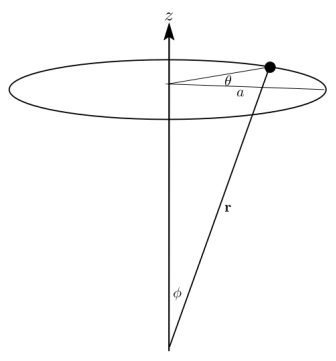
\includegraphics[trim=1.5 0 0 0, height=3.5cm,clip]{11_0.png}
	% 	% \caption{四个区域搜索空间}
  % \end{figure}
  
	\column{0.1\textwidth}

\end{columns}
\end{frame}

%%%%%%%%%%%%%%%%%%%%%%%%%%%%

\begin{frame}
  \frametitle{确定性误差 \hfill 
\includegraphics[height=0.5cm]{00_logo.png}}
  \begin{columns}
    \column{0.1\textwidth}
    
    \column{0.8\textwidth}
    \begin{enumerate}
      \item Bias \quad 理论上,当没有外界作用时,IMU的输出应该为0.但是,实际数据存在一个偏置b,加速度计bias对位姿估计的影响:
      \begin{equation}
        v_{err} = b^a t,\quad p_{err} = \frac{1}{2} b^a t^2        
      \end{equation}

      \item Scale \quad scale可以看成是理论数值和输出值之间的比值,如下图所示.
      \item Nonorthogonality/Misalignment Errors \quad 
      多轴IMU传感器制作的时候,由于制作工艺的问题,会使得xyz轴可能不垂直,如下图所示.

    \end{enumerate}

    \begin{figure}[h]
      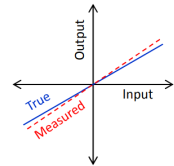
\includegraphics[trim=1.5 0 0 0, height=3.5cm,clip]{11_1.png}
      \qquad
      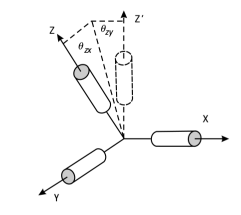
\includegraphics[trim=1.5 0 0 0, height=3.5cm,clip]{11_2.png}

      % \caption{四个区域搜索空间}
    \end{figure}
    % {\color{red}旋转矩阵是一个正交矩阵.它的行列式为1,且每个列向量都是单位向量且相互正交,它的逆等于它的转置.}
    
    \column{0.1\textwidth}
  
  \end{columns}
  \end{frame}   

